\documentclass[xcolor=svgnames]{beamer}
\usepackage[utf8]{inputenc}
\usepackage[czech]{babel}

\newcommand{\semitransp}[2][35]{\color{fg!#1}#2}
\usepackage{wrapfig}
\usepackage{graphicx, booktabs}
\usepackage[autolanguage]{numprint}

\usetheme{Proso}

\title{Co bylo? Co bude?}
\author{Jan Papoušek}
\institute{Fakulta informatiky Masarykovy univerzity}      % Enter your institute name between curly braces
\date{10. 2. 2016}

\begin{document}
% --------------------------- SLIDE --------------------------------------------
\frame[plain]{\titlepage}
% ------------------------------------------------------------------------------
% --------------------------- SLIDE --------------------------------------------
\begin{frame}
	\frametitle{Historie}
	\textbf{jaro, 2013}
		\begin{itemize}
			\item přihlásil jsem se na doktorát\\
				{\tiny o tématu nevím absolutně nic}
		\end{itemize}
	\pause
	\textbf{podzim, 2013}
		\begin{itemize}
			\item všichni řešili věci okolo \url{tutori.fi.muni.cz}
			\item Víťa vytvořil prototyp Slepých map (1.)
			\item já se rozhodl Slepé mapy přepsat (2.)\\
				{\tiny nakonec to umělo to samé jako původní verze}
			\item první a poslední verze adaptivity
		\end{itemize}
	\pause
	\textbf{jaro, 2014}
		\begin{itemize}
			\item první 2 AB experimenty\\
				{\tiny první jsem v záchvatu entuziasmu předčasně ukončil}
			\item začali jsme sbírat hodnocení obtížnosti\\
				{\tiny já jsem byl spíše skeptický}
		\end{itemize}
\end{frame}
% ------------------------------------------------------------------------------
% --------------------------- SLIDE --------------------------------------------
\begin{frame}
	\frametitle{Historie}
	\textbf{podzim, 2014}
		\begin{itemize}
			\item práce na Autoškole chytře
			\item zoufalý boj s daty z AB experimentů
			\item dohodli jsme se s Memorixem na vytvoření Anatoma
		\end{itemize}
	\pause
	\textbf{jaro, 2015}
		\begin{itemize}
			\item práce na proso-apps (Anatom, Slepé mapy)
			\item analýza interakce modelu a algortimu pro konstrukci otázek
		\end{itemize}
	\pause
	\textbf{podzim, 2015}
		\begin{itemize}
			\item nová verze Slepých map (3.)
			\item první verze Anatoma (1.)
			\item \uv{nové} AB experimenty - referenční otázky\\
				{\tiny k referenčním otázkám jsem byl spíše skeptický}
		\end{itemize}
	\pause
	\textbf{jaro, 2016}
		\begin{itemize}
			\item další verze proso-apps\\~~~~$\rightarrow$ nová verze Slepých map (4.) a Anatoma (2.)
			\item nasazení modelu se zapomínáním
		\end{itemize}
\end{frame}
% ------------------------------------------------------------------------------
% --------------------------- SLIDE --------------------------------------------
\begin{frame}[plain]
	\noindent\makebox[\textwidth]{
\includegraphics[width=\paperwidth]{figures/facepalm}}
\end{frame}
% ------------------------------------------------------------------------------
% --------------------------- SLIDE --------------------------------------------
\begin{frame}
	\frametitle{Inženýrské chyby}
	\textbf{neplatný CSRF token}
		\begin{itemize}
			\item pro určitou skupinu uživatelů jsme neukládali odpovědi\\
				~~~~(přišli jsme tak nejméně o 60 000 odpovědí)
		\end{itemize}
	\pause
	\textbf{špatná aktualizace dat v prediktivním modelu}
		\begin{itemize}
			\item například aktualizovaná obtížnost pro Finsko se uložila ke Švédsku
			\item podobné chyby se opakovaly
		\end{itemize}
	\pause
	\textbf{referenční otázka nebyla každá desátá}
		\begin{itemize}
			\item někteří uživatelé měli sérii třeba 10 a více referenčních otázek
		\end{itemize}
\end{frame}
% ------------------------------------------------------------------------------
% --------------------------- SLIDE --------------------------------------------
\begin{frame}[plain]
	\begin{center}
		{\Huge Má to, co děláme, smysl?}
	\end{center}
\end{frame}
% ------------------------------------------------------------------------------
% --------------------------- SLIDE --------------------------------------------
\begin{frame}
	\frametitle{Neformální State of the Art}
	\textbf{prediktivní modely}
		\begin{itemize}
			\item mám offline data a metriku popisující kvalitu predikcí
			\item snažím se vytvořit model, který je lepší\\~~~~(a mohu jej porovnat vůči ostatním)
		\end{itemize}
	\textbf{algoritmy na řízení procvičování}
		\begin{itemize}
			\item mám systém a algoritmus
			\item seženu si lidi, které rozdělím na kontrolní a analyzovanou skupinu
			\item snažím se, aby můj skupina používající můj algoritmus dosahovala
				lepších výsledků než kontrolní skupina (měřeno pre/post testem)
		\end{itemize}
\end{frame}
% ------------------------------------------------------------------------------
% --------------------------- SLIDE --------------------------------------------
\begin{frame}
	\frametitle{Neformální State of the Art}
	jeden z prvních relevantních článků, co jsem četl, k evaluaci adaptivity:
	\begin{itemize}
		\item On the impact of adaptive test question selection for learning efficiency
	\end{itemize}
	\begin{center}
		statický obsah\\vs.\\téměř statický obsah\\vs.\\adaptivní interaktivní obsah (otázky)
	\end{center}
\end{frame}
% ------------------------------------------------------------------------------
% --------------------------- SLIDE --------------------------------------------
\begin{frame}
\begin{center}
	prediktivní model se nezdá být pro procvičování až tak důležitý
\end{center}
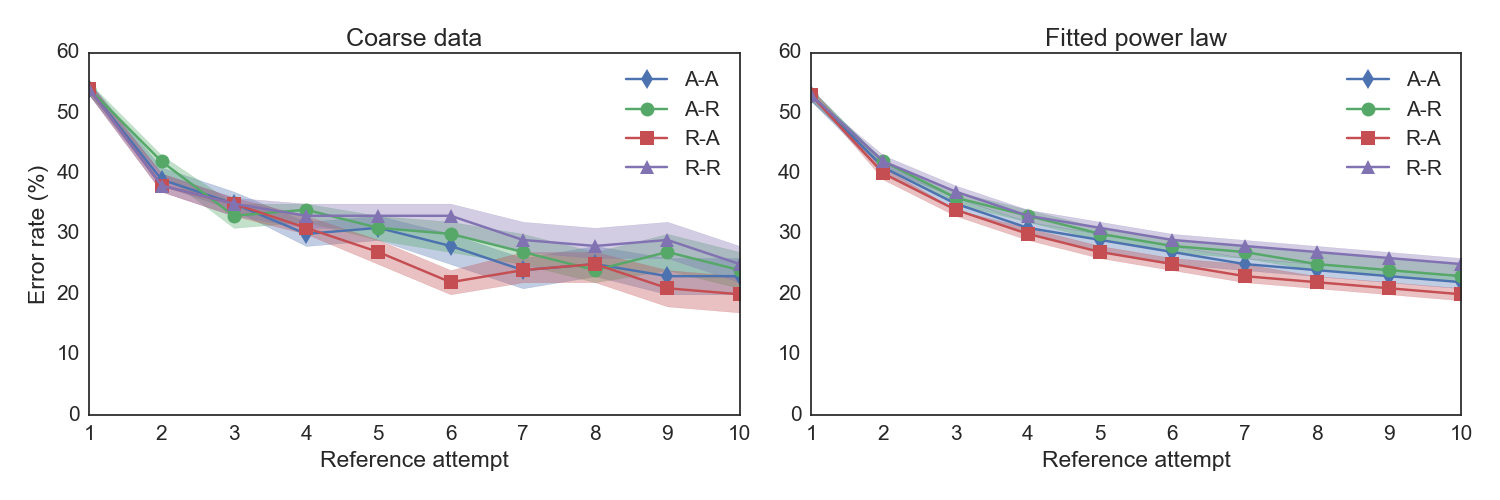
\includegraphics[width=\textwidth]{figures/balanced_global_learning_raw}
\end{frame}
% ------------------------------------------------------------------------------
\begin{frame}
	\frametitle{Disertace: Prediktivní model}
	\begin{center}
		zatím žádný postup

		\bigskip
		cílem je nasadit model se zapomínáním
	\end{center}
\end{frame}
% --------------------------- SLIDE --------------------------------------------
% ------------------------------------------------------------------------------
\begin{frame}
	\frametitle{Disertace: Konstrukce otázek}
	\begin{itemize}
		\item algoritmus implementovaný v proso-apps
		\item výběr položky $\rightarrow$ distraktory
		\item výběr distraktorů na základě historických dat
		\item možná rozšíření (např. regulace obtížnosti distraktorů)
		\item dopad na data a jejich další analýzu
	\end{itemize}
\end{frame}
% --------------------------- SLIDE --------------------------------------------
% ------------------------------------------------------------------------------
\begin{frame}
	\frametitle{Disertace: Evaluace}
	\begin{itemize}
		\item framework pro online evaluaci
		\item možné zkreslení výsledků způsobené odcházením uživatelů ze systému
		\item případové studie:
			\begin{itemize}
				\item adaptivní vs. náhodné procvičování
				\item cílová obtížnost
				\item (obtížnost distraktorů)
			\end{itemize}
	\end{itemize}
\end{frame}
% --------------------------- SLIDE --------------------------------------------
\begin{frame}
	\frametitle{Co bylo dobré udělat?}
	\textbf{podívat se na užitečnost prediktivního modelu}
	\begin{itemize}
		\item AB experiment s více prediktivnímy modely
		\item na učení a čas strávený v systému pravděpodobně malý vliv
		\item důvěra uživatele v systém?
	\end{itemize}
	\pause
	\textbf{porovnat náš přístup k adaptivitě vůči konkurenci}
	\begin{itemize}
		\item AB experiment s více algoritmy pro konstrukci otázek\\
			{\tiny nabízí se porovnání s ACT-R, Leitner systémem, \ldots}
	\end{itemize}
\end{frame}
% ------------------------------------------------------------------------------
\end{document}
